
\section{Sở GD \& ĐT HÀ TĨNH NĂM HỌC 25--26, Lần 1}
\Opensolutionfile{ans}[ans/05-26-2-HaTinh-SoGD-L1-TN]

\caulc 
%%--- Câu 1
\begin{ex}%[Thi thử SGD Hà Tĩnh Lần 1 - 2025-2026]%[Nguyễn Thanh Phong, 26-2-DuAnDeTHPT2025-2026]%[2H2H1-3]
\immini{Cho hình lập phương $ABCD.A'B'C'D'$. Tìm mệnh đề \textbf{sai}?
\choice
{$\left(\overrightarrow{AD};\overrightarrow{A'B'}\right)=90^{\circ}$}
{\True $\left(\overrightarrow{A'A};\overrightarrow{CB'}\right)=45^{\circ}$}
{$\left(\overrightarrow{AB};\overrightarrow{A'C'}\right)=45^{\circ}$}
{$\left(\overrightarrow{AC};\overrightarrow{B'D'}\right)=90^{\circ}$}
}{
\begin{tikzpicture}[scale=0.8, line cap = round, line join = round, font=\footnotesize, >=stealth]
	\def\a{3.5}
	\path 	(0:0) coordinate (A)
	++(0:\a) coordinate (D)
	++(-130:\a/2) coordinate (C)
	($(A)+(C)-(D)$) coordinate (B)
	($(A)+(90:\a)$) coordinate (A')
	($(B)+(90:\a)$) coordinate (B')
	($(C)+(90:\a)$) coordinate (C')
	($(D)+(90:\a)$) coordinate (D');
	\draw[dashed] 	(B)--(A)--(D)	(A)--(A');
	\draw 	(C)--(C') 	(D)--(D') 	(B)--(B') 	(B)--(C)--(D) (A')--(B')--(C')--(D')--cycle;
	\foreach \x/\g in {A/180,B/180,C/0,D/0,A'/180,B'/180,C'/0,D'/0}
	\fill[black] 	(\x) circle (1pt)
	($(\g:4mm)+(\x)$) node {$\x$};
\end{tikzpicture}
}
\loigiai{
Ta có $\overrightarrow{A'A} = \overrightarrow{B'B}$ nên $\left(\overrightarrow{A'A};\overrightarrow{CB'}\right) = \left(\overrightarrow{B'B};\overrightarrow{CB'}\right)$.\\
Vì mặt bên $BCC'B'$ là hình vuông nên $\left(\overrightarrow{B'B};\overrightarrow{CB'}\right) = 180^{\circ} - \widehat{BB'C} = 180^{\circ} - 45^{\circ} = 135^{\circ}$. 
}
\end{ex}

%%--- Câu 2
\begin{ex}%[Thi thử SGD Hà Tĩnh Lần 1 - 2025-2026]%[Nguyễn Thanh Phong, 26-2-DuAnDeTHPT2025-2026]%[2D6H1-2]
Gieo ngẫu nhiên một con xúc xắc cân đối và đồng chất hai lần liên tiếp. Tính xác suất để tổng số chấm xuất hiện trong hai lần gieo bằng $8$ biết rằng lần gieo thứ nhất xuất hiện mặt $5$ chấm.
\choice
{$\dfrac{1}{3}$}
{$\dfrac{5}{6}$}
{$\dfrac{1}{36}$}
{\True $\dfrac{1}{6}$}
\loigiai{
	Gọi biến cố $A$: \lq\lq Lần gieo thứ nhất xuất hiện mặt $5$ chấm\rq\rq. \\
	Tập hợp các kết quả thuận lợi cho $A$ là $A = \{(5;1); (5;2); (5;3); (5;4); (5;5); (5;6)\} \Rightarrow n(A) = 6$. \\
	Gọi biến cố $B$: \lq\lq Tổng số chấm xuất hiện trong hai lần gieo bằng $8$\rq\rq. \\
	Khi đó $A \cap B$ là biến cố: \lq\lq Lần $1$ xuất hiện mặt $5$ chấm và tổng $2$ lần bằng $8$\rq\rq $\Rightarrow A \cap B = \{(5;3)\}$. \\
	Do đó $n(A \cap B) = 1$. \\
	Áp dụng công thức xác suất có điều kiện $\mathrm{P}(B \mid A) = \dfrac{n(A \cap B)}{n(A)} = \dfrac{1}{6}$.
}
\end{ex}

%%--- Câu 3
\begin{ex}%[Thi thử SGD Hà Tĩnh Lần 1 - 2025-2026]%[Nguyễn Thanh Phong, 26-2-DuAnDeTHPT2025-2026]%[2D1N1-2]
Cho hàm số $y=f(x)$ có bảng biến thiên như hình vẽ dưới đây. Hàm số đồng biến trên khoảng nào?
\begin{center}
		
\begin{tikzpicture}[scale=1, line cap = round, line join = round, font=\footnotesize, >=stealth]
			\tkzTabInit[nocadre=false,lgt=1.2,espcl=2.5,deltacl=0.6]
			{$x$/0.6, $f'(x)$/0.6, $f(x)$/2} 
			{$-\infty$, $-3$, $0$, $3$, $+\infty$} 
			\tkzTabLine{,-,0,+,0,-,0,+,} 
			\tkzTabVar{+/ $+\infty$, -/ $-1$, +/ $1$, -/ $-1$ , +/ $+\infty$} 
		\end{tikzpicture}
\end{center}
\choice
{\True $(-3;0)$}
{$(0;+\infty)$}
{$(-\infty;3)$}
{$(-3;3)$}
\loigiai{
	Từ bảng biến thiên, ta thấy hàm số đồng biến trên các khoảng $(-3; 0)$ và $(3; +\infty)$.
}
\end{ex}

%%--- Câu 4
\begin{ex}%[Thi thử SGD Hà Tĩnh Lần 1 - 2025-2026]%[Nguyễn Thanh Phong, 26-2-DuAnDeTHPT2025-2026]%[1D2N3-2]
Cho cấp số nhân $(u_n)$ với $u_1=1$ và $u_2=2$. Công bội của cấp số nhân đã cho là
\choice
{$q=-2$}
{\True $q=2$}
{$q=-\dfrac{1}{2}$}
{$q=\dfrac{1}{2}$}
\loigiai{
	Ta có $u_2 = u_1 \cdot q \Rightarrow q = \dfrac{u_2}{u_1} = \dfrac{2}{1}=2$. 
}
\end{ex}

%%--- Câu 5
\begin{ex}%[Thi thử SGD Hà Tĩnh Lần 1 - 2025-2026]%[Nguyễn Thanh Phong, 26-2-DuAnDeTHPT2025-2026]%[2H5N1-2]
Trong không gian tọa độ $Oxyz$, cho mặt phẳng $(P)\colon x-2y-4=0$, khi đó một véc-tơ pháp tuyến của mặt phẳng $(P)$ là
\choice
{$\overrightarrow{n}=(-1;2;4)$}
{\True $\overrightarrow{n}=(1;-2;0)$}
{$\overrightarrow{n}=(1;-2;-4)$}
{$\overrightarrow{n}=(-1;2;-4)$}
\loigiai{
	Một véc-tơ pháp tuyến của mặt phẳng $(P)\colon x - 2y - 4 = 0$ là $\overrightarrow{n}=(1;-2;0)$.
}
\end{ex}

%%--- Câu 6
\begin{ex}%[Thi thử SGD Hà Tĩnh Lần 1 - 2025-2026]%[Nguyễn Thanh Phong, 26-2-DuAnDeTHPT2025-2026]%[2H2N2-3]
Trong không gian tọa độ $Oxyz$, cho véc-tơ $\overrightarrow{a}$ thỏa mãn $\overrightarrow{a}=4\overrightarrow{i}+3\overrightarrow{j}-5\overrightarrow{k}$. Tọa độ véc-tơ $\overrightarrow{a}$ là
\choice
{$(-5;4;3)$}
{\True $(4;3;-5)$}
{$(-4;-3;5)$}
{$(3;4;-5)$}
\loigiai{
	Ta có $\overrightarrow{a}=4\overrightarrow{i}+3\overrightarrow{j}-5\overrightarrow{k}$ nên tọa độ của véc-tơ $\overrightarrow{a}$ là $(4;3;-5)$.
}
\end{ex}
%%--- Câu 7
\begin{ex}%[Thi thử SGD Hà Tĩnh Lần 1 - 2025-2026]%[Nguyễn Thanh Phong, 26-2-DuAnDeTHPT2025-2026]%[2D4N1-4]
	Cho hàm số $f(x)=3^x+1$. Một nguyên hàm của $f(x)$ trên $\mathbb{R}$ là
	\choice
	{$F(x)=3^x+x$}
	{$F(x)=\dfrac{3^x}{\ln 3}$}
	{$F(x)=3^x \ln 3$}
	{\True $F(x)=\dfrac{3^x}{\ln 3}+x$}
	\loigiai{
		Họ nguyên hàm của hàm số $f(x)$ là $\displaystyle\int (3^x+1)\mathrm{\,d}x = \dfrac{3^x}{\ln 3} + x + C$. \\
		Chọn $C=0$, ta được một nguyên hàm của $f(x)$ là $F(x) = \dfrac{3^x}{\ln 3} + x$.
	}
\end{ex}

%%--- Câu 8
\begin{ex}%[Thi thử SGD Hà Tĩnh Lần 1 - 2025-2026]%[Nguyễn Thanh Phong, 26-2-DuAnDeTHPT2025-2026]%[2D4N2-1]
	Cho hàm số $y=f(x)$ liên tục trên $\mathbb{R}$ thỏa mãn $\displaystyle\int\limits_0^5 f(x)\mathrm{\,d}x=6$, $\displaystyle\int\limits_2^5 f(x)\mathrm{\,d}x=2$. Giá trị của biểu thức $\displaystyle\int\limits_0^2 f(x)\mathrm{\,d}x$ bằng
	\choice
	{$8$}
	{\True $4$}
	{$3$}
	{$2$}
	\loigiai{
Ta có
\allowdisplaybreaks
		\begin{eqnarray*}
			&\displaystyle\int\limits_0^2 f(x)\mathrm{\,d}x + \displaystyle\int\limits_2^5 f(x)\mathrm{\,d}x &= \displaystyle\int\limits_0^5 f(x)\mathrm{\,d}x\\
			\Leftrightarrow &\displaystyle\int\limits_0^2 f(x)\mathrm{\,d}x &= \displaystyle\int\limits_0^5 f(x)\mathrm{\,d}x - \displaystyle\int\limits_2^5 f(x)\mathrm{\,d}x \\
			\Leftrightarrow &\displaystyle\int\limits_0^2 f(x)\mathrm{\,d}x&= 6 - 2 = 4.
		\end{eqnarray*}
	}
\end{ex}

%%--- Câu 9
\begin{ex}%[Thi thử SGD Hà Tĩnh Lần 1 - 2025-2026]%[Nguyễn Thanh Phong, 26-2-DuAnDeTHPT2025-2026]%[1D5H1-3]
	Khảo sát thời gian ứng dụng AI vào học tập trong một ngày của học sinh lớp $12$A, thu được mẫu số liệu như sau:
	\begin{center}
		\begin{tabular}{|c|c|c|c|c|c|}
			\hline
			Thời gian (\textit{phút}) & $[20; 25)$ & $[25; 30)$ & $[30;35)$ & $[35;40)$ & $[40;45)$ \\
			\hline
			Số học sinh & $5$ & $8$ & $14$ & $10$ & $6$ \\
			\hline
		\end{tabular}
	\end{center}
	Số trung bình cộng của mẫu số liệu ghép nhóm trên bằng (\textit{làm tròn kết quả hàng phần trăm})?
	\choice
	{$31{,}95$}
	{$31{,}94$}
	{$32{,}96$}
	{\True $32{,}97$}
	\loigiai{
		Số học sinh (cỡ mẫu) là $n = 5 + 8 + 14 + 10 + 6 = 43$. \\
		Các giá trị đại diện của từng nhóm lần lượt là $22{,}5$; $27{,}5$; $32{,}5$; $37{,}5$; $42{,}5$. \\
		Số trung bình cộng của mẫu số liệu ghép nhóm là
		$$\overline{x} = \dfrac{5 \cdot 22{,}5 + 8 \cdot 27{,}5 + 14 \cdot 32{,}5 + 10 \cdot 37{,}5 + 6 \cdot 42{,}5}{43} = \dfrac{1417{,}5}{43} \approx 32{,}97.$$
	}
\end{ex}

%%--- Câu 10
\begin{ex}%[Thi thử SGD Hà Tĩnh Lần 1 - 2025-2026]%[Nguyễn Thanh Phong, 26-2-DuAnDeTHPT2025-2026]%[1D1N5-3]
	Phương trình $\sin x+1=0$ có nghiệm là
	\choice
	{$x=k\pi$, $k \in \mathbb{Z}$}
	{$x=-\dfrac{\pi}{2}+k\pi$, $k \in \mathbb{Z}$}
	{\True $x=-\dfrac{\pi}{2}+k2\pi$, $k \in \mathbb{Z}$}
	{$x=\pi+k2\pi$, $k \in \mathbb{Z}$}
	\loigiai{
		Ta có $\sin x + 1 = 0 \Leftrightarrow \sin x = -1 \Leftrightarrow x = -\dfrac{\pi}{2} + k2\pi$ ($k \in \mathbb{Z}$).
	}
\end{ex}

%%--- Câu 11
\begin{ex}%[Thi thử SGD Hà Tĩnh Lần 1 - 2025-2026]%[Nguyễn Thanh Phong, 26-2-DuAnDeTHPT2025-2026]%[1D6H4-3]
	Tập nghiệm của bất phương trình $\log_{\tfrac{1}{2}}(x-1)+3>0$ là
	\choice
	{$(-\infty;9)$}
	{$(9;+\infty)$}
	{\True $(1;9)$}
	{$(1;7)$}
	\loigiai{
Ta có
\allowdisplaybreaks
\begin{eqnarray*}
	\heva{&x-1>0\\&\log_{\tfrac{1}{2}}(x-1)+3>0} &\Leftrightarrow \heva{&x>1\\&\log_{\tfrac{1}{2}}(x-1)>-3}\\
	&\Leftrightarrow \heva{&x>1\\&(x-1) < \left(\dfrac{1}{2}\right)^{-3}}\\
	&\Leftrightarrow \heva{&x>1\\&x-1 < 8}\\
	&\Leftrightarrow 1 < x < 9.
\end{eqnarray*}
	}
\end{ex}

%%--- Câu 12
\begin{ex}%[Thi thử SGD Hà Tĩnh Lần 1 - 2025-2026]%[Nguyễn Thanh Phong, 26-2-DuAnDeTHPT2025-2026]%[2D1H3-1]
	Giá trị lớn nhất của hàm số $y=\dfrac{3x+2}{x+1}$ trên đoạn $[0;2]$ bằng
	\choice
	{$\dfrac{10}{3}$}
	{\True $\dfrac{8}{3}$}
	{$3$}
	{$2$}
	\loigiai{
		Ta có $y' = \dfrac{1}{(x+1)^2} > 0$, $\forall x \in [0;2]$. \\
		Suy ra hàm số đồng biến trên đoạn $[0;2]$. \\
		Do đó, giá trị lớn nhất của hàm số trên đoạn $[0;2]$ đạt được tại $x = 2$. \\
		Vậy $\max\limits_{x \in [0;2]} y = y(2) = \dfrac{3 \cdot 2 + 2}{2 + 1} = \dfrac{8}{3}$.
	}
\end{ex}
\Closesolutionfile{ans}
\Opensolutionfile{ans}[ans/05-26-2-HaTinh-SoGD-L1-DS]
\cauds
%%--- Câu 1
\begin{ex}%[Thi thử SGD Hà Tĩnh Lần 1 - 2025-2026]%[Nguyễn Thanh Phong, 26-2-DuAnDeTHPT2025-2026]%[2H5V2-8]
	\immini{
	Trong không gian với hệ tọa độ $Oxyz$, mắt một người quan sát đặt tại điểm $M(1;2;3)$ và quan sát một thanh $AB$ với $A(7;8;-3)$, $B(2;3;-3)$. Một tấm bìa cứng có dạng hình tròn thuộc mặt phẳng $(Oxy)$ có tâm $O(0;0;0)$, bán kính $R$ và che khuất hoàn toàn thanh $AB$ đối với người quan sát tại điểm $M$.
}{
	\begin{tikzpicture}[scale=0.8, font=\footnotesize, line join=round, line cap=round, >=stealth]
		\def\R{1.3}
		\path (-4, -1) coordinate (M) (1.5, 1.5) coordinate (A) (2.5, -0.5) coordinate (B) (0, 0) coordinate (O);
		\path[name path=lineMA] (M) -- (A);
		\path[name path=lineMB] (M) -- (B);
		\path[name path=circleC] (O) circle (\R);
		\draw (M) -- (A) -- (B) (M) -- (B);
		\draw[fill=white] (O) circle (\R);
		\draw [name intersections={of=lineMA and circleC, by={i1,i2}}, dashed] (i1) -- (i2);
		\draw [name intersections={of=lineMB and circleC, by={j1,j2}}, dashed] (j1) -- (j2);
		\foreach \x/\g in {A/45,B/-45,M/90,O/-90}
		\draw[fill=black] (\x) circle (1pt) ($(\g:3mm)+(\x)$) node {$\x$};
		\begin{scope}[shift={(-4.3, -1.8)}, scale=0.45]
			\fill (0, 1.7) circle (0.3);
			\fill[rounded corners=2pt] (-0.3, 0.4) rectangle (0.3, 1.3);
			\draw[line width=4pt, line cap=round] (-0.15, 0.4) -- (-0.2, -0.5) (0.15, 0.4) -- (0.2, -0.5);
			\draw[line width=3pt, line cap=round] (-0.3, 1.2) -- (-0.7, 0.8) -- (-0.35, 0.5) (0.3, 1.2) -- (0.7, 0.8) -- (0.35, 0.5);
		\end{scope}
	\end{tikzpicture}
}
	\choiceTF
	{\True Véc-tơ $\overrightarrow{MA}=(6;6;-6)$}
	{Đường thẳng $AB$ tạo với mặt phẳng chứa tấm bìa một góc $30^{\circ}$}
	{\True Phương trình đường thẳng $MA \colon \heva{&x=1+t \\&y=2+t\\&z=3-t} \ (t \in \mathbb{R})$}
	{\True Tấm bìa có bán kính nhỏ nhất bằng $\sqrt{41}$}
	\loigiai{
		\begin{itemchoice}
			\itemch Ta có $\overrightarrow{MA} = (7-1; 8-2; -3-3) = (6; 6; -6)$.
			\itemch Tấm bìa thuộc mặt phẳng $(Oxy)$ nên mặt phẳng chứa tấm bìa có phương trình $z=0$, nhận $\overrightarrow{k}=(0;0;1)$ làm véc-tơ pháp tuyến. \\
			Ta có $\overrightarrow{AB} = (-5; -5; 0)$. Vì $\overrightarrow{AB} \cdot \overrightarrow{k} = -5 \cdot 0 - 5 \cdot 0 + 0 \cdot 1 = 0$ nên $AB \parallel (Oxy)$. \\
			Do đó, góc giữa đường thẳng $AB$ và mặt phẳng chứa tấm bìa bằng $0^{\circ}$.
			\itemch Đường thẳng $MA$ đi qua $M(1;2;3)$ và có một véc-tơ chỉ phương $\overrightarrow{u} = \dfrac{1}{6}\overrightarrow{MA} = (1; 1; -1)$. \\
			Phương trình tham số của $MA$ là $\heva{&x=1+t \\&y=2+t\\&z=3-t}$ $(t \in \mathbb{R})$.
			\itemch 
\immini{Bóng của đoạn $AB$ in lên mặt phẳng $(Oxy)$ khi chiếu từ $M$ là đoạn thẳng $A'B'$ với $A' = MA \cap (Oxy)$ và $B' = MB \cap (Oxy)$.\\
Vì $A' \in MA$ nên $A'(1+t; 2+t; 3-t)$. Do $A' \in (Oxy)$ nên $z = 3-t=0 \Leftrightarrow t=3 \Rightarrow A'(4;5;0)$.\\
Đường thẳng $MB$ qua $M(1;2;3)$, có véc-tơ chỉ phương $\overrightarrow{MB} = (1; 1; -6)$ có phương trình $\heva{&x=1+k \\&y=2+k\\&z=3-6k} (k\in \mathbb{R})$.\\
}
{
	\begin{tikzpicture}[scale=0.75, line join=round, line cap=round, >=stealth, font=\footnotesize]
    \path 
        (0,0) coordinate (O)
        (4,5) coordinate (A')
        (1.5,2.5) coordinate (B');
    \fill[cyan!10] (O) -- ({sqrt(41)},0) arc (0:90:{sqrt(41)}) -- cycle;

    \draw[step=1cm, gray!40, thin, dashed] (-0.5,-0.5) grid (7,6);
    \draw[red] ({sqrt(41)},0) arc (0:90:{sqrt(41)});
    \draw  (O) -- (B')(A') -- (B');
	\draw[<->](O) -- (A') node[midway, sloped, below] {$R$};
    \foreach \p/\g in {
        O/225, 
        A'/45, 
        B'/135
    }
    \fill (\p) circle (1pt) ($(\g:4mm)+(\p)$) node[black] {$\p$};
	\draw[->] (-0.7,0) -- (7.5,0) node[below] {$x$};
    \draw[->] (0,-0.7) -- (0,6.5) node[left] {$y$};
\end{tikzpicture}
}
Do $B' \in (Oxy)$ nên $z = 3-6k=0 \Leftrightarrow k=\dfrac{1}{2} \Rightarrow B'\left(\dfrac{3}{2}; \dfrac{5}{2}; 0\right)$.\\
Để tấm bìa tâm $O$ che khuất toàn bộ đoạn $A'B'$ thì bán kính $R$ phải lớn hơn hoặc bằng khoảng cách từ $O$ đến mọi điểm trên đoạn $A'B'$.\\
Khoảng cách lớn nhất từ gốc toạ độ đến một đoạn thẳng luôn đạt được tại một trong hai đầu mút. Ta tính
$$ OA' = \sqrt{4^2 + 5^2} = \sqrt{41}; \quad OB' = \sqrt{\left(\dfrac{3}{2}\right)^2 + \left(\dfrac{5}{2}\right)^2} = \dfrac{\sqrt{34}}{2}. $$
Vì $OA' > OB'$ nên $\max\limits_{K \in A'B'} OK = OA' = \sqrt{41}$.\\
Vậy bán kính nhỏ nhất của tấm bìa cần dùng là $R = \sqrt{41}$.
		\end{itemchoice}
	}
\end{ex}
%%--- Câu 2
\begin{ex}%[Thi thử SGD Hà Tĩnh Lần 1 - 2025-2026]%[Nguyễn Thanh Phong, 26-2-DuAnDeTHPT2025-2026]%[2D1V5-8]
	Cho hàm số $y=f(x)=\dfrac{x^2-x+100}{x}$.
	\choiceTF
	{\True Tập xác định của hàm số là $\mathscr{D}=\mathbb{R} \setminus \{0\}$}
	{\True Tiệm cận xiên của đồ thị hàm số $y=f(x)$ là đường thẳng có phương trình $y=x-1$}
	{Hàm số $y=f(x)$ không có điểm cực trị}
	{\True Xí nghiệp $A$ sản xuất $x$ sản phẩm với tổng chi phí được cho bởi công thức $C(x)=x^2-x+100$ (đơn vị ngàn đồng, $x>1$). Khi đó chi phí sản xuất trung bình của một sản phẩm thấp nhất bằng $19$ ngàn đồng}
	\loigiai{
		\begin{itemchoice}
			\itemch Hàm số xác định khi $x \ne 0$. Vậy tập xác định $\mathscr{D}=\mathbb{R} \setminus \{0\}$.
			\itemch Ta có $y = \dfrac{x^2-x+100}{x} = x - 1 + \dfrac{100}{x}$. \\
			Vì $\lim\limits_{x \to \pm\infty} \left[f(x) - (x-1)\right] = \lim\limits_{x \to \pm\infty} \dfrac{100}{x} = 0$ nên đồ thị hàm số có tiệm cận xiên là $y=x-1$.
			\itemch Ta có $y' = 1 - \dfrac{100}{x^2} = 0 \Leftrightarrow x^2 = 100 \Leftrightarrow x = \pm 10$. \\
			Vì đạo hàm đổi dấu khi qua hai điểm $x =- 10$ và $x=10$ nên hàm số có $2$ điểm cực trị.
			\itemch Chi phí sản xuất trung bình cho một sản phẩm là
			$$ \overline{C}(x) = \dfrac{C(x)}{x} = \dfrac{x^2-x+100}{x} = x - 1 + \dfrac{100}{x} \quad (\text{với } x > 1). $$
			Ta có $\overline{C}'(x) = 1 - \dfrac{100}{x^2} = 0 \Rightarrow x = 10$ (do $x > 1$). \\
			Bảng biến thiên của hàm số $\overline{C}(x)$ trên khoảng $(1; +\infty)$
			\begin{center}
				
\begin{tikzpicture}[scale=1, line cap = round, line join = round, font=\footnotesize, >=stealth]
					\tkzTabInit[nocadre=false, lgt=1.5, espcl=2.5, deltacl=0.6]
					{$x$/0.6, $\overline{C}'(x)$/0.7, $\overline{C}(x)$/2}
					{$1$, $10$, $+\infty$}
					\tkzTabLine{ , -, 0, +, }
					\tkzTabVar{+/ $100$, -/ $19$, +/ $+\infty$}
				\end{tikzpicture}
			\end{center}
			Dựa vào bảng biến thiên, ta thấy $\min\limits_{x \in (1; +\infty)} \overline{C}(x) = \overline{C}(10) = 19$. \\
			Vậy chi phí sản xuất trung bình thấp nhất là $19$ ngàn đồng.
		\end{itemchoice}
	}
\end{ex}
%%--- Câu 3
\begin{ex}%[Thi thử SGD Hà Tĩnh Lần 1 - 2025-2026]%[Nguyễn Thanh Phong, 26-2-DuAnDeTHPT2025-2026]%[0D0V2-4]
	Từ một nhóm học sinh gồm $6$ học sinh lớp $10$A, $8$ học sinh lớp $10$B và $7$ học sinh lớp $10$C. Chọn ngẫu nhiên $5$ học sinh từ nhóm học sinh trên.
	\choiceTF
	{\True Số cách chọn $5$ học sinh tùy ý là $20\,349$ cách}
	{Số cách chọn $5$ học sinh có đủ cả ba lớp sao cho số học sinh lớp $10$C lớn hơn hai là $1\,860$ cách}
	{\True Số cách chọn $5$ học sinh đều thuộc lớp $10$A là $6$ cách}
	{\True Xác suất để chọn $5$ học sinh sao cho không tồn tại lớp nào có đúng $1$ học sinh được chọn là $\dfrac{1\,528}{6\,783}$}
	\loigiai{
		Tổng số học sinh là $6+8+7=21$ học sinh.
		\begin{itemchoice}
			\itemch Số cách chọn $5$ học sinh tùy ý là $\mathrm{C}_{21}^5 = 20\,349$ cách. 
			\itemch Chọn $5$ học sinh có đủ $3$ lớp mà số học sinh lớp $10$C lớn hơn $2$. Do đó, số học sinh lớp $10$C chỉ có thể là $3$ (vì nếu là $4$ thì chỉ còn $1$ suất cho $2$ lớp kia nên không đủ $3$ lớp). \\
			Suy ra mỗi lớp $10$A và $10$B phải có đúng $1$ học sinh. \\
			Số cách chọn là $\mathrm{C}_7^3 \cdot \mathrm{C}_6^1 \cdot \mathrm{C}_8^1 = 35 \cdot 6 \cdot 8 = 1\,680$. 
			\itemch Số cách chọn $5$ học sinh đều thuộc lớp $10$A là $\mathrm{C}_6^5 = 6$ cách. 
			\itemch Gọi biến cố $A$: \lq\lq Không tồn tại lớp nào có đúng $1$ học sinh được chọn\rq\rq. \\
			Điều này có nghĩa là số học sinh được chọn từ mỗi lớp phải thuộc tập $\{0; 2; 3; 4; 5\}$. Vì tổng số học sinh là $5$ nên ta có các trường hợp sau:
			\begin{itemize}
				\item \textbf{Trường hợp 1:} Chọn $5$ học sinh từ đúng $1$ lớp. \\
				Số cách: $\mathrm{C}_6^5 + \mathrm{C}_8^5 + \mathrm{C}_7^5 = 6 + 56 + 21 = 83$ cách.
				\item \textbf{Trường hợp 2:} Chọn từ $2$ lớp, gồm $1$ lớp chọn $3$ học sinh và $1$ lớp chọn $2$ học sinh. Số cách:
				\begin{itemize}
					\item Lớp $10$A và $10$B: $\mathrm{C}_6^3\cdot\mathrm{C}_8^2 + \mathrm{C}_6^2\cdot\mathrm{C}_8^3 = 20\cdot 28 + 15\cdot 56 = 1\,400$.
					\item Lớp $10$B và $10$C: $\mathrm{C}_8^3\cdot\mathrm{C}_7^2 + \mathrm{C}_8^2\cdot\mathrm{C}_7^3 = 56\cdot 21 + 28\cdot 35 = 2\,156$.
					\item Lớp $10$C và $10$A: $\mathrm{C}_7^3\cdot\mathrm{C}_6^2 + \mathrm{C}_7^2\cdot\mathrm{C}_6^3 = 35\cdot 15 + 21\cdot 20 = 945$.
				\end{itemize}
				Tổng của trường hợp $2$ là $1\,400 + 2\,156 + 945 = 4\,501$ cách.
			\end{itemize}
			Số kết quả thuận lợi cho biến cố $A$ là $n(A) = 83 + 4\,501 = 4\,584$. \\
			Xác suất cần tìm là $\mathrm{P}(A) = \dfrac{4\,584}{20\,349} = \dfrac{1\,528}{6\,783}$. 
		\end{itemchoice}
	}
\end{ex}

%%--- Câu 4
\begin{ex}%[Thi thử SGD Hà Tĩnh Lần 1 - 2025-2026]%[Nguyễn Thanh Phong, 26-2-DuAnDeTHPT2025-2026]%[2D4V3-5]
	Chiếc mũ rộng vành được mô hình hóa khi cho hình phẳng $(H)$ được giới hạn bởi đồ thị hàm số $y=f(x)=\begin{cases} \sqrt{1-x^2} & \text{khi } -1 \le x \le 0 \\ x^3+1 & \text{khi } 0 < x \le 1 \end{cases}$, trục $Ox$ và các đường thẳng $x=-1$, $x=1$ quay xung quanh trục $Ox$ (tham khảo hình vẽ). Biết đơn vị trên mỗi trục là dm.
	\begin{center}
%\begin{tikzpicture}[scale=0.5, font=\footnotesize, line join=round, line cap=round, transform shape]

%    \shade[inner color=gray!10, outer color=gray!70, draw=black!80, thick] 
%        (-4.5, -0.5) .. controls (-4.5, -1.8) and (-2.5, -2.2) .. (0, -2.2) 
%        .. controls (2.5, -2.2) and (4.5, -1.8) .. (4.5, -0.5) 
%        .. controls (4.5, 0.5) and (2.5, 1) .. (0, 1) 
%        .. controls (-2.5, 1) and (-4.5, 0.5) .. (-4.5, -0.5);
%
%    \fill[pattern=crosshatch dots, pattern color=black!40] 
%        (-4.5, -0.5) .. controls (-4.5, -1.8) and (-2.5, -2.2) .. (0, -2.2) 
%        .. controls (2.5, -2.2) and (4.5, -1.8) .. (4.5, -0.5) 
%        .. controls (4.5, 0.5) and (2.5, 1) .. (0, 1) 
%        .. controls (-2.5, 1) and (-4.5, 0.5) .. (-4.5, -0.5);
%
%    \shade[top color=white, bottom color=gray!60, draw=black!80, thick] 
%        (-2.2, 0) .. controls (-2.2, 2.5) and (-1.5, 3.5) .. (0, 3.5) 
%        .. controls (1.5, 3.5) and (2.2, 2.5) .. (2.2, 0) 
%        arc (0:-180:2.2 and 0.8);
%
%    \fill[pattern=crosshatch dots, pattern color=black!40] 
%        (-2.2, 0) .. controls (-2.2, 2.5) and (-1.5, 3.5) .. (0, 3.5) 
%        .. controls (1.5, 3.5) and (2.2, 2.5) .. (2.2, 0) 
%        arc (0:-180:2.2 and 0.8);
%
%    \draw[double=white, double distance=5pt, draw=black!80, thick] 
%        (-2.2, 0.02) arc (-180:0:2.2 and 0.8);
%        
%    \draw[black!70, thick] (-2.2, 0.02) arc (-180:0:2.2 and 0.8);
%
%\end{tikzpicture}
%\quad
\begin{tikzpicture}[scale=1.5, font=\footnotesize, line join=round, line cap=round, >=stealth]

    \fill[pattern=crosshatch dots, pattern color=gray!80] 
        (-1,0) arc (180:90:1) -- (0,0) -- cycle;
        
    \fill[pattern=crosshatch dots, pattern color=gray!80] 
        (0,0) -- (0,1) -- plot[domain=0:1, samples=100] (\x, {\x^3 + 1}) -- (1,0) -- cycle;

    \draw[->] (-1.5,0) -- (1.5,0) node[above] {$x$};
    \draw[->] (0,-0.5) -- (0,2.5) node[right] {$y$};
    

    \draw[thick] (-1,0) arc (180:90:1);
    \draw[thick, smooth, samples=100, domain=0:1] plot (\x, {\x^3 + 1});

    \draw[dashed] (1,0) -- (1,2) -- (0,2);
    \draw[fill=black] (0,0) circle (0.7pt) node[below left] {$O$};
    \draw[fill=black] (-1,0) circle (0.7pt) node[below] {$-1$};
    \draw[fill=black] (1,0) circle (0.7pt) node[below] {$1$};
    \draw[fill=black] (0,2) circle (0.7pt) node[left] {$2$};

    \draw (-1,0) -- (1,0);
    \draw (1,0) -- (1,2); 

    \node[align=left, font=\tiny] (note1) at (-1.5, 2) 
        {$y = \sqrt{1-x^2}$ \\[0.1cm] khi $-1 \le x \le 0$};
    \draw[->] (-0.6, 0.8)--($(note1)+(-0,-0.5)$);
    
    \node[align=left, font=\tiny] (note2) at (1.5, 2.5) 
        {$y = x^3 + 1$ \\[0.1cm] khi $0 \le x \le 1$};
    \draw[->] (0.8, 1.5)--($(note2.west)+(0.5,-0.25)$);

\end{tikzpicture}
\quad 
		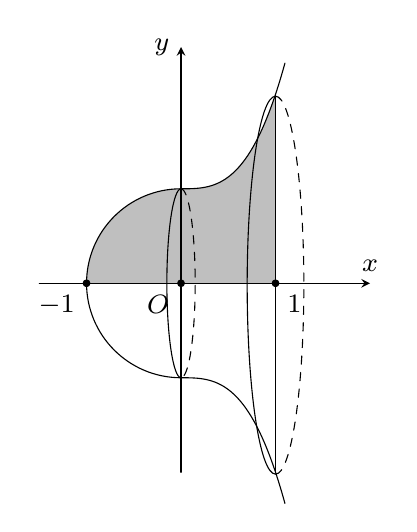
\begin{tikzpicture}[scale=1.2, font=\footnotesize, line cap=round, line join=round, >=stealth, transform shape]
    
    \fill[gray!50] (-1,0) arc (180:90:1)
          -- plot[domain=0:1, variable=\x, samples=50] (\x, {\x^3 + 1})
          -- (1,2)--(1,0)--cycle;

    \draw[->] (-1.5,0) -- (2,0) node[above] {$x$};
    \draw[->] (0,-2) -- (0,2.5) node[left] {$y$};
    
    \draw (-1,0) arc (180:90:1);
    \draw plot[domain=0:1.1, variable=\x, samples=100] (\x, {\x^3 + 1});
    \draw (1,2) -- (1,-2);
    \draw (-1,0) arc (-180:-90:1);
    \draw plot[domain=0:1.1, variable=\x, samples=100] (\x, {-(\x^3 + 1)});
    
    \draw (0, 1) arc (90:270:0.15 and 1);
	\draw[dashed] (0, 1) arc (90:-90:0.15 and 1); 
    \draw (1, 1.98) arc (90:270:0.3 and 2); 
	\draw [dashed] (1, 1.98) arc (90:-90:0.3 and 2); 
    
    \draw[fill=black] (0,0) circle (1pt) node[below left] {$O$};
    \draw[fill=black] (-1,0) circle (1pt) node[below left]{$-1$};
    \draw[fill=black] (1,0) circle (1pt) node[below right] {$1$};
\end{tikzpicture}
	\end{center}
	\choiceTF
	{Diện tích của hình phẳng $(H)$ là $S=\displaystyle\int\limits_{-1}^1 \left|\sqrt{1-x^2}+x^3+1\right|\mathrm{\,d}x$}
	{\True Thể tích của khối tròn xoay trên là $\dfrac{97}{42}\pi$ (dm$^3$)}
	{\True Giá trị của hàm số $f(x)$ khi $x=1$ bằng $2$}
	{Vành của chiếc mũ (giao tuyến của mặt tròn xoay cắt bởi mặt phẳng vuông góc với trục $Ox$ tại $x=1$) có diện tích bằng $2\pi$ (dm$^2$)}
	\loigiai{
		\begin{itemchoice}
			\itemch Diện tích hình phẳng $(H)$ được tính bằng tổng tích phân trên hai đoạn
			$$ S = \displaystyle\int\limits_{-1}^0 \sqrt{1-x^2} \mathrm{\,d}x + \displaystyle\int\limits_0^1 (x^3+1) \mathrm{\,d}x $$
			\itemch Thể tích khối tròn xoay là
			\allowdisplaybreaks
			\begin{eqnarray*}
				V &=& \pi \displaystyle\int\limits_{-1}^0 \left(\sqrt{1-x^2}\right)^2 \mathrm{\,d}x + \pi \displaystyle\int\limits_0^1 (x^3+1)^2 \mathrm{\,d}x \\
				&=& \pi \displaystyle\int\limits_{-1}^0 (1-x^2) \mathrm{\,d}x + \pi \displaystyle\int\limits_0^1 (x^6+2x^3+1) \mathrm{\,d}x \\
				&=& \pi \left( x - \dfrac{x^3}{3} \right)\Bigg|_{-1}^0 + \pi \left( \dfrac{x^7}{7} + \dfrac{x^4}{2} + x \right)\Bigg|_0^1 \\
				&=& \pi \left[ 0 - \left(-1+\dfrac{1}{3}\right) \right] + \pi \left( \dfrac{1}{7} + \dfrac{1}{2} + 1 \right) \\
				&=& \pi \left( \dfrac{2}{3} + \dfrac{23}{14} \right) = \dfrac{97}{42}\pi \ (\text{dm}^3).
			\end{eqnarray*}
			\itemch Vì $x=1 > 0$ nên $f(1) = 1^3 + 1 = 2$.
			\itemch Giao tuyến của mặt tròn xoay khi cắt bởi mặt phẳng $x=1$ (vuông góc với trục $Ox$) là một hình tròn có bán kính $r = f(1) = 2$. \\
			Diện tích của giao tuyến này là $S' = \pi r^2 = \pi \cdot 2^2 = 4\pi$ (dm$^2$). 
		\end{itemchoice}
	}
\end{ex}
\Closesolutionfile{ans}
\caukq
\Opensolutionfile{ans}[ans/05-26-2-HaTinh-SoGD-L1-TLN]
%%--- Câu 1
\begin{ex}%[Thi thử SGD Hà Tĩnh Lần 1 - 2025-2026]%[Nguyễn Thanh Phong, 26-2-DuAnDeTHPT2025-2026]%[1D6V2-4]
	\textbf{Tỉ lệ lạm phát} là tỉ lệ phần trăm biểu thị mức tăng chung của giá hàng hóa và dịch vụ trong một khoảng thời gian (\textit{thường tính theo năm}). Nếu tỉ lệ lạm phát của năm sau so với năm trước là $i$ thì $A$ đồng ở năm trước tương đương với $P=A(1+i)$ đồng ở năm sau.\\
	Ông An gửi vào ngân hàng $100$ triệu đồng với lãi suất $6\%$/năm, theo hình thức lãi kép, tính lãi mỗi năm một lần (\textit{tức là lãi của năm trước được nhập vào vốn để tính lãi cho năm sau}). Sau $2$ năm, ông An nhận cả vốn và lãi. Giả sử trong $2$ năm đó, tỉ lệ lạm phát ổn định $4\%$/năm. Nếu quy đổi theo mức giá tại thời điểm gửi tiền thì số tiền ông An nhận được sau $2$ năm tương đương bao nhiêu triệu đồng (\textit{làm tròn kết quả đến hàng đơn vị})?
	\shortans{104}
	\loigiai{
		Số tiền (cả vốn và lãi) ông An thực nhận từ ngân hàng sau $2$ năm gửi lãi kép là
		$$ S = 100 \cdot (1 + 6\%)^2 = 112{,}36 \text{ (triệu đồng).} $$
		Theo giả thiết, $A$ đồng ở năm trước tương đương $A(1+i)$ đồng ở năm sau. Do đó, để quy đổi số tiền $P$ từ năm thứ $n$ về giá trị tương đương ở thời điểm ban đầu (năm $0$), ta chia số tiền đó cho $(1+i)^n$. \\
		Vậy, số tiền ông An nhận được sau $2$ năm nếu quy đổi theo mức giá tại thời điểm gửi tiền (với mức lạm phát $4\%$/năm) là
		$$ X = \dfrac{112{,}36}{(1 + 4\%)^2} = \dfrac{112{,}36}{1{,}0816} \approx 104 \text{ (triệu đồng).} $$
}
\end{ex}

%%--- Câu 2
\begin{ex}%[Thi thử SGD Hà Tĩnh Lần 1 - 2025-2026]%[Nguyễn Thanh Phong, 26-2-DuAnDeTHPT2025-2026]%[2D4V2-6]
	Trong một chương trình giao lưu âm nhạc đón tết vui xuân, ban đầu với sự tham dự của $1\,700$ khán giả. Ban tổ chức đã thống kê được số lượng khán giả ở lại sân khấu xem âm nhạc theo thời gian, được mô tả bởi một hàm số liên tục trên $t \in [0;+\infty)$ $$f'(t)=\begin{cases} 1\,700-400t, & 0 \le t \le 2 \\ a(t-2)^2+b, & t>2 \end{cases}$$ (trong đó $f'(t)$ là số khán giả, $t$ là số giờ kể từ khi chương trình bắt đầu, $a$, $b$ là tham số thực), với hàm số $f(t)$ mô tả tổng sự hiện diện của khán giả theo thời gian $t$. Sau $2$ giờ $30$ phút số lượng khán giả ở lại sân khấu là $875$. Hỏi từ khi bắt đầu cho đến khi khán giả ra về hết, trung bình mỗi giờ còn bao nhiêu khán giả ở lại tham gia chương trình âm nhạc?
	\shortans{880}
	\loigiai{
		Vì hàm số $f'(t)$ liên tục trên $[0;+\infty)$ nên nó liên tục tại $t=2$. \\
		Ta có $$\heva{&\lim\limits_{t \to 2^-} f'(t) = 1\,700 - 400 \cdot 2 = 900\\&\lim\limits_{t \to 2^+} f'(t) = a(2-2)^2 + b = b\\&f(2)= 1\,700 - 400 \cdot 2 = 900.}$$
		Do đó, $b = 900$. \\
		Sau $2$ giờ $30$ phút ($t = 2{,}5$ giờ), số lượng khán giả ở lại là $875$ nên
		$$ f'(2{,}5) = 875 \Leftrightarrow a(2{,}5-2)^2 + 900 = 875 \Leftrightarrow 0{,}25a = -25 \Leftrightarrow a = -100. $$
		Vậy hàm số biểu diễn số lượng khán giả là
		$$ f'(t) = \begin{cases} 1\,700-400t & \text{khi } 0 \le t \le 2 \\ -100(t-2)^2+900 & \text{khi } t>2. \end{cases} $$
		Khán giả ra về hết khi $f'(t) = 0$. \\
		Với $t>2$, ta có $-100(t-2)^2+900 = 0 \Leftrightarrow (t-2)^2 = 9 \Rightarrow t-2 = 3 \Leftrightarrow t = 5$ (giờ). \\
		Từ khi bắt đầu đến khi khán giả ra về hết kéo dài $5$ giờ. \\
		Tổng sự hiện diện của khán giả trong $5$ giờ là $\displaystyle\int\limits_0^5 f'(t) \mathrm{\,d}t$. Ta có
		\allowdisplaybreaks
		\begin{eqnarray*}
			\displaystyle\int\limits_0^5 f'(t) \mathrm{\,d}t &=& \displaystyle\int\limits_0^2 (1\,700-400t) \mathrm{\,d}t + \displaystyle\int\limits_2^5 \left[-100(t-2)^2+900\right] \mathrm{\,d}t \\
			&=& \left( 1\,700t - 200t^2 \right)\Bigg|_0^2 + \left[ -\dfrac{100(t-2)^3}{3} + 900t \right]\Bigg|_2^5 \\
			&=& (3\,400 - 800) + \left[ \left( -900 + 4\,500 \right) - (0 + 1\,800) \right] \\
			&=& 2\,600 + 1\,800 = 4\,400.
		\end{eqnarray*}
		Trung bình mỗi giờ có số khán giả ở lại là 
		$$ \dfrac{4\,400}{5} = 880 \text{ (khán giả).} $$
	}
\end{ex}

%%--- Câu 3
\begin{ex}%[Thi thử SGD Hà Tĩnh Lần 1 - 2025-2026]%[Nguyễn Thanh Phong, 26-2-DuAnDeTHPT2025-2026]%[1D7V2-8]
	%Em có sửa lại điều kiện của a, b là a, b >0 thay vì a, b \in \mathbb{R} để khi mẫu thức luôn được xác định và số lượng tế bào luôn là 1 số dương.
	Giả sử số lượng tế bào của một quần thể nấm men tại môi trường nuôi cấy trong phòng thí nghiệm được mô hình hóa bằng hàm số $P(t)=\dfrac{a}{b+\mathrm{e}^{-0{,}75t}}$ (với $a$, $b >0$), trong đó thời gian $t$ được tính bằng giờ. Đạo hàm của hàm số $y=P(t)$ biểu thị tốc độ sinh trưởng của nấm men (tính bằng tế bào/giờ) tại thời điểm $t$ (giờ). Tại thời điểm ban đầu $t=0$, quần thể có $24$ tế bào và tốc độ sinh trưởng là $8$ tế bào/giờ. Sau một thời gian về lâu dài thì số lượng tế bào của quần thể nấm men tiến về giá trị bao nhiêu?
	\shortans{43{,}2}
	\loigiai{
		Tại thời điểm ban đầu $t=0$, quần thể có $24$ tế bào nên
		$$ P(0) = 24 \Leftrightarrow \dfrac{a}{b + \mathrm{e}^0} = 24 \Leftrightarrow \dfrac{a}{b + 1} = 24 \Rightarrow a = 24(b + 1). \quad (1) $$
		Đạo hàm của hàm số $P(t)$ là
		$$ P'(t) = \dfrac{-a \cdot \left(-0{,}75\mathrm{e}^{-0{,}75t}\right)}{\left(b + \mathrm{e}^{-0{,}75t}\right)^2} = \dfrac{0{,}75a \cdot \mathrm{e}^{-0{,}75t}}{\left(b + \mathrm{e}^{-0{,}75t}\right)^2}. $$
		Tại thời điểm $t=0$, tốc độ sinh trưởng là $8$ tế bào/giờ nên
		$$ P'(0) = 8 \Leftrightarrow \dfrac{0{,}75a}{(b + 1)^2} = 8 \Rightarrow 0{,}75a = 8(b + 1)^2. \quad (2) $$
		Thay $(1)$ vào $(2)$, ta được
		$$ 0{,}75 \cdot 24(b + 1) = 8(b + 1)^2 \Leftrightarrow 18(b + 1) = 8(b + 1)^2. $$
		Vì $b + 1 \neq 0$, ta chia cả hai vế cho $8(b + 1)$
		$$ \dfrac{18}{8} = b + 1 \Leftrightarrow 2{,}25 = b + 1 \Leftrightarrow b = 1{,}25. $$
		Suy ra $a = 24 \cdot (1{,}25 + 1) = 54$. \\
		Số lượng tế bào về lâu dài chính là giới hạn của hàm số $P(t)$ khi $t \to +\infty$
		$$ \lim\limits_{t \to +\infty} P(t) = \lim\limits_{t \to +\infty} \dfrac{54}{1{,}25 + \mathrm{e}^{-0{,}75t}}= \dfrac{54}{1{,}25 + 0} = 43{,}2.$$
		Vậy về lâu dài, số lượng tế bào của quần thể tiến về giá trị $43{,}2$.
	}
\end{ex}
%%--- Câu 4
\begin{ex}%[Thi thử SGD Hà Tĩnh Lần 1 - 2025-2026]%[Nguyễn Thanh Phong, 26-2-DuAnDeTHPT2025-2026]%[2H2V2-5]
	Trong không gian tọa độ $Oxyz$, cho hai đường thẳng có phương trình $d \colon \dfrac{x-2}{3}=\dfrac{y-1}{4}=\dfrac{z+5}{5}$; $d' \colon \dfrac{x-1}{a}=\dfrac{y+1}{b}=\dfrac{z+4}{c}$, trong đó $a$, $b$, $c$ là các số thực khác $0$ sao cho các đường thẳng $d$ và $d'$ cắt nhau tại $M$. Mặt phẳng $(P) \colon 2x+y-2z-6=0$ lần lượt cắt các trục $Ox$, $Oy$, $Oz$ tại $A$, $B$, $C$. Tính thể tích của khối tứ diện $MABC$.
	\shortans{13{,}5}
	\loigiai{
	\begin{center}
		\begin{tikzpicture}[
    scale=1, 
    line join=round, line cap=round, font=\footnotesize, >=stealth,
    x={(-0.6cm, -0.4cm)}, 
    y={(1cm, 0cm)}, 
    z={(0cm, 1cm)}
]
    \path 
        (0,0,0) coordinate (O)
        (3,0,0) coordinate (A)
        (0,4,0) coordinate (B)
        (0,0,-2.5) coordinate (C)
        (1,1,2.5) coordinate (M)
        ($(M) + (-1.5, 2, 0)$) coordinate (d1)
        ($(M) + (1.5, -2, 0)$) coordinate (d2)
        ($(M) + (1, 2, 0.5)$) coordinate (d'1)
        ($(M) + (-1, -2, -0.5)$) coordinate (d'2)
		($(M)+(0,0,-3.5)$) coordinate (H)
		;
    \draw[->] (O) -- (4,0,0) node[below] {$x$};
    \draw[->] (O) -- (0,5,0) node[below] {$y$};
    \draw[->] (O) -- (0,0,3) node[left] {$z$};
    \fill[cyan!20, opacity=0.6] (A) -- (B) -- (C) -- cycle;
    \draw[thick] (A) -- (B) -- (C) -- cycle (M) -- (C);
    \draw[dashed] (A) -- (O) (B) -- (O) (C) -- (O) (M)--(H);
    \draw[thick, red] (d1) -- (d2) node[above] {$d$};
    \draw[thick, orange] (d'1) -- (d'2) node[above] {$d'$};
    \draw[thick] (M) -- (A) (M) -- (B);
    \foreach \x/\g in {O/135, A/135, B/45, C/-90, M/90,H/-45}
        \fill[black] (\x) circle (1.5pt) ($(\g:3mm)+(\x)$) node {$\x$};
\end{tikzpicture}
	\end{center}
		Mặt phẳng $(P)$ cắt các trục $Ox$, $Oy$, $Oz$ lần lượt tại $A$, $B$, $C$ nên
		$A(3;0;0)$, $B(0;6;0)$ và $C(0;0;-3)$. \\
		Đường thẳng $d$ đi qua điểm $N(2;1;-5)$ và có véc-tơ chỉ phương $\overrightarrow{u} = (3;4;5)$. \\
		Mặt phẳng $(P)$ (cũng là mặt phẳng $(ABC)$) có véc-tơ pháp tuyến $\overrightarrow{n} = (2;1;-2)$. \\
		Ta có $\overrightarrow{u} \cdot \overrightarrow{n} = 3 \cdot 2 + 4 \cdot 1 + 5 \cdot (-2) = 0$. \\
		Lại có điểm $N(2;1;-5) \in d$ nhưng không thuộc $(P)$ vì $2\cdot 2 + 1 - 2\cdot (-5) - 6 = 9 \ne 0$. \\
		Suy ra đường thẳng $d$ song song với mặt phẳng $(ABC)$. \\
		Vì hai đường thẳng $d$ và $d'$ cắt nhau tại $M$ nên $M \in d$. \\
		Do $d \parallel (ABC)$ nên khoảng cách từ $M$ đến mặt phẳng $(ABC)$ bằng khoảng cách từ điểm $N$ đến $(ABC)$. Chiều cao của tứ diện $MABC$ từ đỉnh $M$ là
		$$ h = \mathrm{d}(M, (ABC)) = \mathrm{d}(N, (P)) = \dfrac{|2 \cdot 2 + 1 - 2 \cdot (-5) - 6|}{\sqrt{2^2 + 1^2 + (-2)^2}} = \dfrac{9}{3} = 3. $$
		Ta có $\overrightarrow{AB} = (-3;6;0)$ và $\overrightarrow{AC} = (-3;0;-3)$. \\
		Suy ra $\left[\overrightarrow{AB}, \overrightarrow{AC}\right] = (-18; -9; 18)$. \\
		Diện tích tam giác $ABC$ là
		$$ S_{\triangle ABC} = \dfrac{1}{2} \left|\left[\overrightarrow{AB}, \overrightarrow{AC}\right]\right| = \dfrac{1}{2} \sqrt{(-18)^2 + (-9)^2 + 18^2} = \dfrac{27}{2}. $$
		Thể tích của khối tứ diện $MABC$ là
		$$ V = \dfrac{1}{3} \cdot S_{\triangle ABC} \cdot h = \dfrac{1}{3} \cdot \dfrac{27}{2} \cdot 3 = \dfrac{27}{2} = 13{,}5. $$
	}
\end{ex}

%%--- Câu 5
\begin{ex}%[Thi thử SGD Hà Tĩnh Lần 1 - 2025-2026]%[Nguyễn Thanh Phong, 26-2-DuAnDeTHPT2025-2026]%[0D0C2-9]
	Xếp $8$ quyển sách giống nhau vào một giá sách gồm $10$ ngăn. Gọi $P$ là xác suất để xếp $8$ quyển sách vào $10$ ngăn sao cho số quyển sách trong mỗi ngăn không quá $2$ quyển sách, có $4$ ngăn hoặc $6$ ngăn chứa đúng $1$ quyển sách và các ngăn liền kề với ngăn chứa $2$ quyển sách là ngăn không có quyển sách nào. Tính $12\,155P$.
	\shortans{131}
	\loigiai{
		Gọi $x_i$ ($x_i \ge 0$, $x_i \in \mathbb{N}$) là số sách xếp vào ngăn thứ $i$ ($i = 1, \dots, 10$). \\
		Số phần tử của không gian mẫu bằng số nghiệm nguyên không âm của phương trình
		$$x_1 + x_2 + \dots + x_{10} = 8.$$
		Suy ra $n(\Omega) = \mathrm{C}_{8+10-1}^8 = \mathrm{C}_{17}^8 = 24\,310$. \\
		Gọi $A$ là biến cố cần tính xác suất. Vì các quyển sách là giống nhau, ta quy bài toán về việc tìm các dãy gồm $10$ phần tử thuộc tập $\{0; 1; 2\}$ (tương ứng với số sách trong mỗi ngăn). \\
		Giả sử trong $10$ ngăn có $n_0$ ngăn chứa $0$ quyển, $n_1$ ngăn chứa $1$ quyển và $n_2$ ngăn chứa $2$ quyển sách. \\
		Do đó, ta có hệ phương trình sau  $\heva{&n_0+n_1+n_2=10 \\ &1\cdot n_1 + 2\cdot n_2 = 8.}$ \\
		Theo giả thiết, $n_1 \in \{4; 6\}$. Ta xét hai trường hợp
		\begin{itemize}
			\item \textbf{Trường hợp 1:} $n_1 = 4 \Rightarrow n_2 = 2$ và $n_0 = 4$. \\
			Ta coi $4$ ngăn chứa $0$ quyển sách là các vách ngăn xếp thành một hàng, tạo ra $5$ khoảng trống (bao gồm $2$ khoảng ở hai đầu và $3$ khoảng ở giữa). \\
			Vì ngăn chứa $2$ quyển sách chỉ được kề với ngăn $0$ quyển nên mỗi ngăn chứa $2$ quyển phải đứng đơn độc trong $1$ khoảng trống. \\
			Ta chọn $2$ khoảng trống để đặt $2$ ngăn chứa $2$ quyển sách có $\mathrm{C}_5^2 = 10$ cách. \\
			Còn lại $3$ khoảng trống, ta đem $4$ ngăn chứa $1$ quyển sách xếp vào $3$ khoảng trống này. \\
			Số cách xếp tương đương số nghiệm nguyên không âm của phương trình $a+b+c=4$. Ta có $$\mathrm{C}_{4+3-1}^4 = \mathrm{C}_6^4 = 15 \text{ cách}.$$
			Số cách xếp thỏa mãn \textbf{TH1} là $10 \cdot 15 = 150$ cách.
			\item \textbf{Trường hợp 2:} $n_1 = 6 \Rightarrow n_2 = 1$ và $n_0 = 3$. \\
			Ta có $3$ ngăn chứa $0$ quyển sách tạo thành $4$ khoảng trống. \\
			Chọn $1$ khoảng trống để đặt duy nhất $1$ ngăn chứa $2$ quyển sách có $\mathrm{C}_4^1 = 4$ cách. \\
			Còn lại $3$ khoảng trống, ta xếp $6$ ngăn chứa $1$ quyển sách vào $3$ khoảng trống này. \\
			Số cách xếp tương đương số nghiệm nguyên không âm của phương trình $a+b+c=6$. Ta có $$\mathrm{C}_{6+3-1}^6 = \mathrm{C}_8^6 = 28 \text{ cách}.$$ 
			Số cách xếp thỏa mãn \textbf{TH2} là $4 \cdot 28 = 112$ cách.
		\end{itemize}
		Số kết quả thuận lợi cho biến cố $A$ là $n(A) = 150 + 112 = 262$. \\
		Xác suất của biến cố $A$ là $\mathrm{P}(A) = \dfrac{n(A)}{n(\Omega)} = \dfrac{262}{24\,310} = \dfrac{131}{12\,155}$. \\
		Vậy $12\,155P = 12\,155 \cdot \dfrac{131}{12\,155} = 131$.
	}
\end{ex}

%%--- Câu 6
\begin{ex}%[Thi thử SGD Hà Tĩnh Lần 1 - 2025-2026]%[Nguyễn Thanh Phong, 26-2-DuAnDeTHPT2025-2026]%[1H8V7-9]
	\immini{
	Một giàn khung thép đỡ bồn nước sinh hoạt có dạng là hình lăng trụ tam giác đều $ABC.A'B'C'$. Để giàn đỡ có kết cấu chắc chắn người ta hàn thêm $1$ số thanh sắt (hình vẽ), trong đó có hai thanh $AB' \perp BC'$. Cho biết cạnh đáy của giàn đỡ $AB=2\text{ (m)}$. Tính thể tích $V$ (m$^3$) của khối lăng trụ $ABC.A'B'C'$ (\textit{kết quả làm tròn đến hàng phần trăm}).
	}{
		\begin{tikzpicture}[scale=0.8, font=\footnotesize, line cap=round, line join=round, >=stealth]
			\tikzset{
				bonnuoc/.style={
					line cap=round, line join=round
				}
			}
			
			\newcommand{\bonnuoc}[5]{%
				\fill[gray!20]
				(#1-#3, #2) rectangle (#1+#3, #2+#5);
				\fill[gray!20]
				(#1-#3,#2) arc(180:360:#3 and #4)
				--(#1+#3,#2) -- cycle;
				\fill[black,opacity=.13]
				(#1-#3,#2) rectangle (#1-#3+.4,#2+#5);
				\fill[black,opacity=.13]
				(#1+#3,#2) rectangle (#1+#3-.45,#2+#5);
				\draw[dashed,bonnuoc,black!65]
				(#1-#3,#2) arc(180:0:#3 and #4);
				\pgfmathsetmacro{\stripBot}{#2+#5*.35}
				\pgfmathsetmacro{\stripTop}{#2+#5*.52}
				\fill[cyan!80]
				(#1-#3,\stripBot) arc(180:360:#3 and #4)
				--(#1+#3,\stripTop)
				arc(360:180:#3 and #4) -- cycle;
				\draw[bonnuoc,blue!60!black]
				(#1-#3,\stripBot) arc(180:360:#3 and #4);
				\draw[bonnuoc,blue!60!black]
				(#1-#3,\stripTop) arc(180:360:#3 and #4);
				\node[text=white,
				font=\bfseries\small,
				inner sep=2.5pt, rounded corners=2pt]
				at (#1,{(3*\stripBot+\stripTop)/5}) {HOÀN MỸ};
				\draw[bonnuoc,gray!75!black]
				(#1-#3,#2+.4) arc(180:360:#3 and #4);
				\draw[bonnuoc,gray!75!black]
				(#1-#3,#2+.65) arc(180:360:#3 and #4);
				\draw[bonnuoc,gray!75!black]
				(#1-#3,#2+#5-.5) arc(180:360:#3 and #4);
				\draw[bonnuoc,gray!75!black]
				(#1-#3,#2+#5-.7) arc(180:360:#3 and #4);
				\fill[gray!40] (#1,#2+#5) ellipse(#3 and #4);
				\draw[bonnuoc,black!80]
				(#1,#2+#5) ellipse(#3 and #4);
				\draw[bonnuoc,black!80]
				(#1-#3,#2) arc(180:360:#3 and #4);
				\draw[bonnuoc,black!80]
				(#1-#3,#2)--(#1-#3,#2+#5);
				\draw[bonnuoc,black!80]
				(#1+#3,#2)--(#1+#3,#2+#5);
			}
			\tikzset{
				langTruKhuat/.style={dashed, thick},
				langTruLien/.style={thick}
			}
			
			\newcommand{\langTru}[3]{
				\path
				(0.2,0)              coordinate (A)
				++(#1,0)            coordinate (C)
				++({-150}:3*#1/4)   coordinate (B)
				($(A)+(0,#2)$)      coordinate (Ap)
				($(B)+(0,#2)$)      coordinate (Bp)
				($(C)+(0,#2)$)      coordinate (Cp)
				($(A)!#3!(Ap)$)     coordinate (M)
				($(C)!#3!(Cp)$)     coordinate (N)
				($(B)!#3!(Bp)$)     coordinate (K)
				;
				\draw[langTruKhuat] (A)--(C) (B)--(Bp) (M)--(N);
				\draw[langTruLien]   (A)--(Ap) (C)--(Cp);
				\draw[langTruLien]   (A)--(B)--(C);
				\draw[langTruLien]   (Ap)--(Bp)--(Cp)--cycle;
				\draw[langTruLien]   (M)--(K)--(N);
				\foreach \pt/\pos/\name in {A/left/A, B/below/B, C/right/C, Ap/left/A', Bp/above/B', Cp/right/C'} {
					\draw[fill=black] (\pt) circle (1pt) node[\pos] {$\name$};
				}
				\draw[fill=black] (M) circle(1pt) (N) circle(1pt) (K) circle(1pt);
			}
			\bonnuoc{2.15}{-0.55}{1.35}{0.55}{4.5}
			\langTru{4.5}{4.5}{0.4}
		\end{tikzpicture}
	}
	\shortans{2{,}45}
\loigiai{
\immini{
	Gọi $h$ là chiều cao của lăng trụ. Ta có $\overrightarrow{BB'} = \overrightarrow{CC'}$ và $\overrightarrow{BB'} \perp (ABC)$.\\
	Vì $AB' \perp BC'$ nên $\overrightarrow{AB'} \cdot \overrightarrow{BC'} = 0$. Ta có
	\allowdisplaybreaks
	\begin{eqnarray*}
		& \left(\overrightarrow{AB} + \overrightarrow{BB'}\right)\cdot\left(\overrightarrow{BC} + \overrightarrow{CC'}\right) &= 0 \\
		\Leftrightarrow  & \left(\overrightarrow{AB} + \overrightarrow{BB'}\right)\cdot\left(\overrightarrow{BC} + \overrightarrow{BB'}\right) &= 0 \\
		\Leftrightarrow  & \overrightarrow{AB}\cdot\overrightarrow{BC} + \overrightarrow{AB}\cdot\overrightarrow{BB'} + \overrightarrow{BB'}\cdot\overrightarrow{BC} + \overrightarrow{BB'}^2 &= 0.
	\end{eqnarray*}
	Do $\overrightarrow{BB'} \perp (ABC)$ nên $\overrightarrow{AB}\cdot\overrightarrow{BB'} = 0$ và $\overrightarrow{BB'}\cdot\overrightarrow{BC} = 0$. \\
	Lại có góc giữa hai véc-tơ $\overrightarrow{AB}$ và $\overrightarrow{BC}$ là $180^{\circ} - 60^{\circ} = 120^{\circ}$. Suy ra
	$$ AB \cdot BC \cdot \cos 120^{\circ} + h^2 = 0 \Leftrightarrow 2 \cdot 2 \cdot \left(-\dfrac{1}{2}\right) + h^2 = 0 \Rightarrow h = \sqrt{2}. $$
	Thể tích khối lăng trụ là
	$$ V = S_{ABC} \cdot h = \dfrac{2^2\sqrt{3}}{4} \cdot \sqrt{2} = \sqrt{6} \approx 2{,}45 \text{ (m}^3). $$
}{
	\begin{tikzpicture}[scale=0.8, line cap=round, line join=round, font=\footnotesize, >=stealth]
		\def\a{4}
		\def\h{4.5}
		\path 	(0:0) coordinate (A)
		++(0:\a) coordinate (C)
		++(-150:3*\a/4) coordinate (B)
		($(A)+(90:\h)$) coordinate (A')
		($(B)+(90:\h)$) coordinate (B')
		($(C)+(90:\h)$) coordinate (C');
		\draw[dashed,thick] (A)--(C);
		\draw[thick] (C)--(C') (B)--(B') (A)--(A') (A)--(B)--(C) (A')--(B')--(C')--cycle;
		\draw[thick, blue] (A)--(B') (B)--(C'); % Vẽ thêm 2 thanh sắt chéo nhau
		\foreach \x/\g in {A/180,B/-45,C/0,A'/180,B'/-45,C'/0}
		\draw[fill=black] (\x) circle (1pt) ($(\g:4mm)+(\x)$) node {$\x$};
	\end{tikzpicture}
}
}
\end{ex}
\Closesolutionfile{ans}
% \indapan{4}{ans/05-26-2-HaTinh-SoGD-L1}